\chapter{Side-channel attacks}
	I \emph{side-channel attacks}\index{Side-channel attacks} sono metodi di criptanalisi che sfruttano le side-channels informations insieme ad altre tecniche di analisi per recuperare la chiave utilizzata da un \disps\cite{standaert2010introduction}.
	
	\begin{figure}
		\begin{center}
			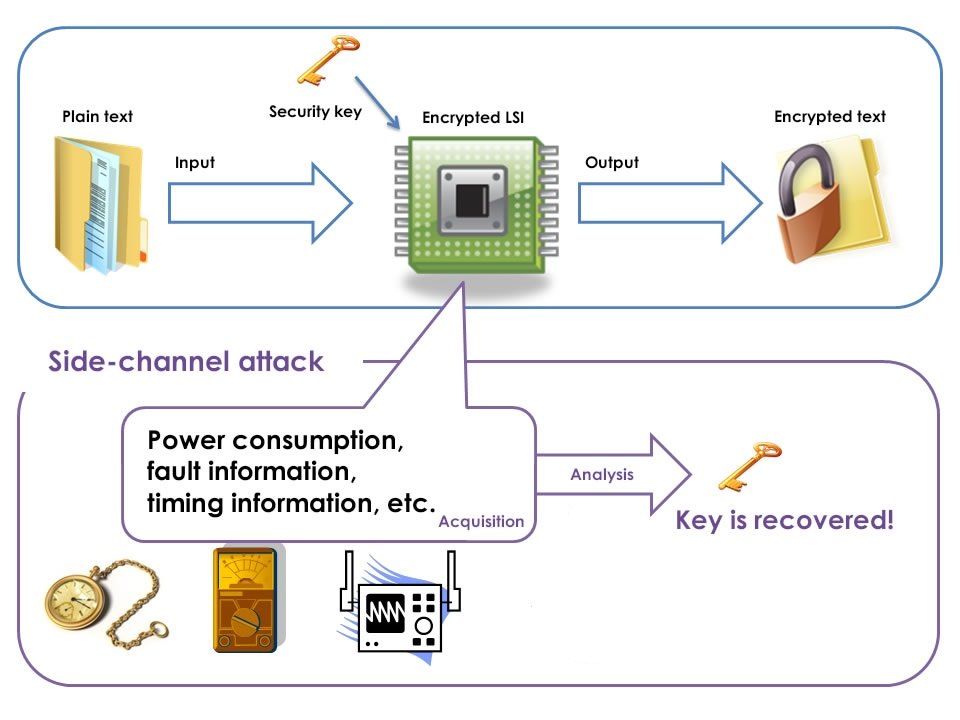
\includegraphics[scale=.4]{side-channel-attack_large}
			\caption{Esempio di side-channel attack}
			\label{fig:attack}
		\end{center}
	\end{figure}
	
	Nella \cref{fig:attack} si può vedere una configurazione tipo di side-channel attack. Da una parte c'è il dispositivo che implementa la funzione crittografica e accanto c'è lo strumento utilizzato per rilevare le grandezze fisiche prodotte dal dispositivo attaccato. La cosa fondamentale è che questo tipo di attacchi non vanno a colpire direttamente la funzione crittografica ma sfruttano le informazioni fisiche dell'ambiente intorno al dispositivo.
	
	L'analisi di questi metodi ha acquisito notevole interesse dato che questo tipo di attacchi possono essere montati velocemente e molto spesso non richiedono hardware particolare e costoso. Con pochi euro si possono ad esempio acquistare in comuni negozi di bricolage o elettronica apparecchi in grado di analizzare il consumo elettrico di un dispositivo. Con tali apparecchi è possibile montare in pochi secondi un attacco di tipo \emph{Simple Power Analysis}\cite{mangard2002simple} che verrà spiegato più avanti. 
	
	Il governo degli USA, nel suo "Orange book"\cite{latham1986department} indica dei requisiti di sicurezza per i sistemi operativi. Questo documento introduce i primi standard per l'\emph{information leakage}. Purtroppo la letteratura specializzata è però molto variegata e disomogenea quindi, come prima cosa, cerchiamo di trovare un modo per classificare i vari tipi di attacchi in maniera tale da avere una visione più sistemistica del settore.
	
	\section{Classificazione degli attacchi}	
		Le caratteristiche che contraddistinguono ogni singolo attacco sono molteplici e differenti tra loro. In questa sezione si cercherà di raggruppare e definire quelle più importanti ed associabili alla maggior parte degli attacchi.
	
		\subsection*{Tipi di canali}	
			Nel lavoro di \emph{Ge, Yarom, Cock e Heiser}\cite{ge2016survey} vengono fornite alcune definizioni che utilizzeremo nel prosieguo di questa tesi. La prima distinzione che è necessario fare è quella tra side-channel\index{Side-channel} e \emph{covert-channel}\index{Covert channel}. Con i primi ci si riferisce ai canali che lasciano \emph{accidentalmente} filtrare informazioni sensibili (ad esempio una chiave crittografica) in una comunicazione tra due partecipanti fidati. I secondi sono quelli creati e sfruttati dall'attaccante ad esempio tramite l'utilizzo di Trojan e che \emph{deliberatamente} lasciano filtrare le informazioni. In questo lavoro verranno trattati solamente i primi.
			
			L'altra differenza fondamentale per quello che riguarda i canali è quella tra canali di tipo \emph{storage}\index{Storage channel} e canali di tipo \emph{timing}\index{Timing channel}. I canali di tipo storage vengono sfruttati per ottenere qualcosa di direttamente visibile nel sistema (valore dei registri, valore di ritorno di una system call, ecc.). Quelli di tipo timing vengono sfruttati andando ad osservare variazioni del tempo di esecuzione di un programma (o di parti di esso).
			
		\subsection*{Tipi di attacco}		
			\emph{Standaert} nel suo lavoro \cite{standaert2010introduction} utilizza altre due dimensioni interessanti per classificare questi attacchi; l'\emph{invasività}\index{Invasività} e l'\emph{attività/passività}\index{Attività/passività}. 
			
			Si definisce invasivo un attacco che richiede un disassemblamento del dispositivo attaccato per avere accesso diretto ai suoi componenti interni (wiretapping o sensori collegati direttamente all'hardware). Un attacco non invasivo, al contrario, sfrutta solamente le informazioni disponibili esternamente (quasi sempre involontarie) come il tempo d'esecuzione o l'energia consumata.
			
			Si definisce attivo un attacco che cerca di interferire con il corretto funzionamento del dispositivo (fault-injection)\cite{giraud2004dfa,karri2001fault} mentre un attacco passivo si limita ad osservare il comportamento del dispositivo durante il suo lavoro senza disturbarlo. 
			
		\subsection*{Grandezza fisica osservata}		
			Una caratteristica principale di questi attacchi è sicuramente la grandezza fisica che viene osservata per montare l'attacco. Teoricamente, qualunque grandezza fisica misurabile può essere sfruttata ma alcune si prestano maggiormente rispetto ad altre. 
			
			Il tempo e il consumo energetico sono le più sfruttate ma non sono di certo le uniche. \emph{Genkin, Shamir e Tromer} nel loro lavoro \cite{genkin2014rsa} vanno ad ascoltare i rumori prodotti dal processore. \emph{Ferrigno e Hlavac}\cite{ferrigno2008aes} osservano la luce (qualche fotone) emessa dai transistor nel passaggio di stato da 0 a 1. \emph{Martinasek, Zeman e Trasy}\cite{martinasek2012simple} sfruttano i campi elettromagnetici creati dai chip. \emph{Murdoch}, attraverso le variazioni delle frequenze del clock, ricava informazioni sulla temperatura ambientale e cerca di localizzare geograficamente il dispositivo della vittima.
			
			Questo elenco assolutamente non esaustivo delle tecniche utilizzate può far capire quanto variegato ed eterogeneo (nonché in continua evoluzione) sia questo settore.
			
		\subsection*{Hardware attaccato}		
			Gli attacchi possono essere suddivisi anche in base alla componente hardware che viene attaccata. Anche in questo caso ci sono componenti più attaccati (ed attaccabili) di altri (cache e processori) ma non mancano esempi di attacchi a monitor\cite{van1985electromagn}, tastiere\cite{asonov2004keyboard} o stampanti\cite{backes2010acoustic}.
			
		\subsection*{Algoritmo attaccato}		
			Un'ultima classificazione può essere effettuata andando a discriminare gli attacchi secondo l'algoritmo crittografico attaccato. In questo caso i due maggiori algoritmi attaccati sono senza dubbio AES\cite{standard2001announcing} ed RSA\cite{rivest1978method} nelle loro implementazioni più comuni. Altri algoritmi attaccati sono El-Gamal\cite{elgamal1985public} e le curve ellittiche\cite{koblitz1987elliptic,miller1985use}.
			\begin{table}[]
				\scriptsize
				\centering
				\begin{tabular}{|c|c|c|c|c|c|c|c|} \hline
					Articolo					& Grandezza					& Componente	& Algoritmo			& Invasivo	& Attivo	& Canale	& Anno	\\ \hline \hline
					\cite{genkin2014rsa}		& Suono						& CPU			& RSA				& No		& No		& -			& 2014	\\ \hline
					\cite{ferrigno2008aes}		& Luce						& Transistor	& AES				& Sì		& No		& -			& 2008	\\ \hline
					\cite{van1985electromagn}	& Campo elettromagnetico	& Monitor    	& -					& No		& No		& -			& 1985	\\ \hline
					\cite{kocher2018spectre}	& Tempo						& Cache			& RSA				& No		& No		& Timing	& 2018	\\ \hline
					\cite{giraud2004dfa}		& -							& -				& AES				& No		& Sì		& Storage	& 2004	\\ \hline
					\cite{mangard2002simple}	& Consumo elettrico			& Smartcard		& AES				& No		& No		& -			& 2002	\\ \hline
					\cite{asonov2004keyboard}	& Suono						& Tastiere		& -					& No		& No		& -			& 2004	\\ \hline
					\cite{zhou2018efficient}	& Tempo						& Cache			& OpenSSL			& No		& No		& Timing	& 2018	\\ \hline
					\cite{martinasek2012simple}	& Campo elettromagnetico	& Chip			& AES				& No		& No		& -			& 2012	\\ \hline
					\cite{yarom2014flush+}		& Tempo						& Cache			& RSA				& No		& No		& Timing	& 2014	\\ \hline
					\cite{karri2001fault}		& -							& -				& AES				& No		& Sì		& Storage	& 2001	\\ \hline
					\cite{backes2010acoustic}	& Suono						& Stampanti		& -					& No		& No		& -			& 2010	\\ \hline
					\cite{lipp2016armageddon}	& Tempo						& Cache			& AES				& No		& No		& Timing	& 2016	\\ \hline
					\cite{murdoch2006hot}		& Temperatura				& Clock			& -					& No		& No		& -			& 2006	\\ \hline
					\cite{genkin2018drive}		& Tempo						& Browser		& Curve ellittiche	& No		& No		& Timing	& 2018	\\ \hline
				\end{tabular}
				\caption{Classificazione dei principali attacchi conosciuti}
				\label{tab:attacchi}
			\end{table}
			Nella \cref{tab:attacchi} sono classificati con i criteri sopra definiti i principali attacchi conosciuti.
			
			Passiamo adesso ad una breve panoramica sui maggiori attacchi per ogni tipo di grandezza fisica attaccata. Si ricorda che gli attacchi basati sul tempo, categoria nella quale ricadono la maggior parte degli attacchi eseguiti contro le cache, verranno approfonditi nel prossimo capitolo.
			
	\section{Attacchi basati sul suono}\index{Acoustic attacks}
	L'analisi di suoni prodotti da dispositivi meccanici, specialmente in campo militare, risalgono a molto indietro quando si riusciva a distinguere un aereo o una nave a seconda del rumore che produceva.
	
	Anche i dispositivi elettronici, in generale, emettono un grande numero di rumori diversi. Se ad esempio pensiamo ad un computer portatile, alcune informazioni banali che possiamo ricavare dai suoni emessi sono ad esempio l'attività dell'Hard Disk che ci suggerisce un utilizzo della memoria oppure l'accendersi di una ventola che ci suggerisce un intenso utilizzo della CPU. Questo tipo di informazioni sono però troppo generiche specialmente in un dispositivo general purpose che esegue molti processi diversi parallelamente.
	
	Per approfondire il livello di informazione ricevuto le strade più percorse sono due. Aumentare la sensibilità dell'ascoltatore cercando di trovare differenze tra rumori che sembrano uguali o ascoltare rumori più particolari.
	
	\subsection{Differenziazione dei rumori}	
		Uno degli esempi più importanti di questo tipo di attacco è quello eseguito sulle stampanti a matrice di aghi nel 2010\cite{backes2010acoustic}. Il fatto che questo tipo di stampanti sia ormai sparito dall'utilizzo del privato cittadino non deve far pensare ad un attacco anacronistico. Questa scelta è infatti dovuta al fatto che in quell'anno circa il $60\%$ dei medici in Germania e il $30\%$ delle banche utilizzavano ancora quel tipo di stampanti. Alcuni stati europei richiedono per legge l'utilizzo di stampanti a matrici di aghi per la prescrizione di particolari medicine\cite{bernatzky2011schmerzbehandlung}.
		
		\begin{figure}
			\begin{center}
				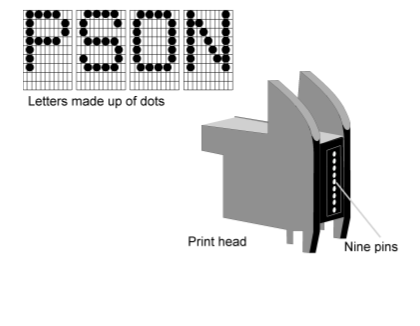
\includegraphics[scale=.5]{printMatrix}
				\caption{Modalità di stampa di una stampante ad aghi}
				\label{fig:matrixHead}
			\end{center}
		\end{figure}
		
		Come si vede in \cref{fig:matrixHead}, una stampante ad aghi scompone ogni lettera in colonne di punti ed utilizza gli aghi necessari per incidere la traccia corretta sulla carta. Lo studio dimostra come sia possibile addestrare una rete neurale per riconoscere il rumore emesso ad ogni singolo passo che cambia in base a quanti e quali aghi vengono utilizzati. Tale rete neurale riconosce il $72\%$ delle parole stampate senza alcuna ulteriore assunzione ed arriva al $95\%$ se si assume una conoscenza del contesto.
		
		L'idea di base è la stessa utilizzata anche in \cite{asonov2004keyboard} nel 2004 per riconoscere i rumori prodotti dai tasti premuti su di una tastiera.
	
	\subsection{Cogliere rumori impercettibili}	
		In questa seconda categoria uno dei principali rappresentati è sicuramente l'attacco\cite{genkin2014rsa} del 2014 portato contro il circuito di regolazione del voltaggio dei computer. Tale circuito è composto da bobine e condensatori che vibrano nel tentativo di fornire un voltaggio costante alla CPU.
		
		Eseguire ad esempio RSA con chiavi differenti provoca pattern di esecuzione di operazioni della CPU diversi che portano all'utilizzo di quantità di energia elettrica differente. Il regolatore di voltaggio reagisce di conseguenza causando fluttuazioni di elettricità che provocano vibrazioni meccaniche nei componenti elettronici e queste vibrazioni vengono trasmesse attraverso l'aria come onde sonore. Il riconoscimento di questi pattern differenti permette agli autori di recuperare la chiave RSA utilizzata.
		
		La particolarità interessante di questo attacco è che non richiede un'attrezzature complessa ed avanzata. Il risultato migliore viene ovviamente ottenuto con un microfono direzionale professionale posizionato ad una distanza di 4 metri dal computer attaccato ma lo stesso risultato viene ottenuto anche con l'utilizzo di un semplice smartphone posto a 30 cm dallo stesso computer.
		
	\subsection{Possibili contromisure}	
		Le possibili contromisure a questo tipi di attacchi sono molteplici e sono sia fisiche che algoritmiche.
		
		\subsubsection*{Insonorizzazione}			
			La prima ovvia soluzione potrebbe essere quella di insonorizzare il dispositivo ad esempio ponendolo dentro a contenitori studiati appositamente. Il problema di questa soluzione è la difficoltà di ottenere un ricircolo d'aria per il raffreddamento. Le aperture per le ventole di raffreddamento sono infatti la fonte di emanazione di questi rumori e non possono essere rimosse facilmente. 
			
			Una soluzione potrebbe essere un contenitore insonorizzato e sigillato dotato di un circuito di raffreddamento a liquido. Questo ovviamente porta ad un notevole innalzamento dei costi del dispositivo.
			
		\subsubsection*{Ambiente rumoroso}		
			Un'altra semplice idea è quella di posizionare il dispositivo in un ambiente rumoroso (all'aperto o in stanze rumorose). Neanche questa soluzione sembra però funzionare perché i rumori "normali" sono concentrate su frequenze più basse rispetto a quelli di interesse e possono essere facilmente filtrati.
			
		\subsubsection*{Randomizzazione}		
			La soluzione migliore è algoritmica e prevede una randomizzazione dell'input. Se parliamo di RSA ad esempio possiamo pensare di non decifrare direttamente il ciphertext ma di modificarlo sommandoci un valore casuale che poi verrà sottratto in maniera opportuna. 
			
			Similmente si può aggiungere un valore casuale al modulo rendendolo ogni volta diverso.
			
	\section{Attacchi basati sulla luce}\index{Optical attacks}
		
	\subsection{Possibili contromisure}	
	\lipsum[1-5]
	\section{Attacchi basati sul consumo elettrico}\index{Power analysis attacks}
	\lipsum[1-5]
	\subsection{Possibili contromisure}	
	\lipsum[1-5]
	\section{Attacchi basati sul campo elettromagnetico}\index{Electromagnetic attacks}
	\lipsum[1-5]
	\subsection{Possibili contromisure}	
	\lipsum[1-5]
	\section{Attacchi basati sulla temperatura}\index{Temperature attacks}
	\lipsum[1-5]
	\subsection{Possibili contromisure}	
	\lipsum[1-5]
	\section{Attacchi fault-based}\index{Fault-based attacks}
	\lipsum[1-5]
	\subsection{Possibili contromisure}	
	\lipsum[1-5]
	\subsection{Possibili contromisure}	
	\lipsum[1-5]